\chapter{Oasis Lib}
\label{ch:Lib}
In this chapter we describe the library of the administration module, called Oasis Lib. The Oasis Lib is the library, which works as a connection between the Oasis Local Db (see \autoref{ch:Db}) and the applications, which runs on the GIRAF system, by providing an API, which the GIRAF applications can use. First the structure of Oasis Lib is described in section \vref{sec:Structure}. Then the implementation of the Oasis Lib is described in \autoref{sec:LibImp}.

\section{Structure}
\label{sec:Structure}
The structure of the Oasis Lib, have been inspired of the MVC pattern, where the system is divided into three parts; Model, View, and Controller. 

In Oasis Lib the Model part is a package containing model objects. Each model object represent a table in the Oasis Local Db.
The model objects is used to encapsulate the data, which is to be saved and loaded from the Oasis Local Db.
The reason that we use model objects is to ease it for the users of the library and to make a uniform way of saving and loading data.
The models can be seen in \autoref{fig:models}.
\begin{figure}
	\centering
		\includegraphics[width=\textwidth]{images/models.png}
	\caption{The models in the Oasis library}
	\label{fig:controllers}
\end{figure}

The controller part is the package containing all the methods, which the developers can use to interact with Oasis Local Db.
The controller methods have been divided into several classes.
The division can be seen in \autoref{fig:controllers}
\begin{figure}
	\centering
		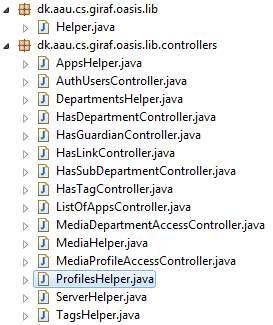
\includegraphics[width=\textwidth]{images/controllers.png}
	\caption{The controllers in the Oasis library}
	\label{fig:controllers}
\end{figure}

They are divided by the models that manipulate, this means that for each table in the db there is a model and a controller.
This gives a good overview that helps the programmers that use the library.

In the library there are no direct reference to the views from the MVC pattern.
This is because the individual applications in the GIRAF system is seen as a view and they have the same function as a view.

\section{Implementation}
\label{sec:LibImp}
Many methods have been inplemented in the library in order to ease the access to the database to as few method calls as possible.
Therefore the code for all the implemented methods will not be show in this section.
The code not shown in this section can be seen in the source code on the attached CD-Rom.


As an example on the implementation of the library the methods \texttt{autenticateProfile} and \texttt{getProfileById} will be presented.

The method \texttt{autenticateProfile} is used to authenticate a profile in order to decide what informations the user should be allowed access to.

First the method verifies that input is not \texttt{null} and that the certificate conformes to the rules for the certificates, if the certificate is rejected \texttt{null} is returned to indicate this.

After the certificate has been verified the profile id will be retrived from the database, if and only if a profile exists with that certificate.
In case a profile exist with the certificate the id will be returned and the profile model will be retrieved from the database.
If no profile with the certificate exists \texttt{-1} will be returned and no profile model will be retrieved.

The code for \texttt{autenticateProfile} can be seen in \autoref{lst:authenticateProfile_implementation}.

\begin{Java}{This is the code for the \texttt{authenticateProfile} method.}{lst:authenticateProfile_implementation}
public Profile authenticateProfile(String certificate) {
	if (certificate == null || !certificate.matches("[a-z]{200}")) {
		return null;
	}

	Profile profile = null;
	long id = au.getIdByCertificate(certificate);

	if (id != -1) {
		profile = getProfileById(id);
	}

	return profile;
}
\end{Java}

The method \texttt{getProfileById} is used the retrieve a profile model from the database.
The model is retrived useing the profile id as a key to get the model by.

First it must be ensured that the id is above zero, as the database can not handle zero or negative values.
After this check the database is queried to retrive the profile model.
A conversion is needed as the database returns a Cursor obejct and this object must be converted into a profile model. kilde: http://developer.android.com/reference/android/database/Cursor.html
This conversion is done in the auxiliry method \texttt{cursorToProfile}, which maps values in the Cursor to values in the profile model.
If the Cursor from the database is null or empty no profile was found in the database.

The code for \texttt{getProfileById} method can be seen in \autoref{lst:getProfileById_implementation}.

\begin{Java}{This is the code for the \texttt{getProfileById} method.}{lst:getProfileById_implementation}
public Profile getProfileById(long id) {
	Profile profile = null;
	
	if (id <= 0) {
		return null;
	}
	
	Uri uri = ContentUris.withAppendedId(ProfilesMetaData.CONTENT_URI, id);
	Cursor c = _context.getContentResolver().query(uri, columns, null, null, null);

	if (c != null) {
		if (c.moveToFirst()) {
			profile = cursorToProfile(c);
		}
		c.close();
	}

	return profile;
}
\end{Java}

For further information on how the Oasis library's methods work, see the JavaDoc which is place on the appended CD-Rom.